\documentclass[11pt, a4paper]{article}
\usepackage[a4paper, margin=1in]{geometry}


\usepackage{adjustbox}
\usepackage{mathtools}
\usepackage{amsmath}
\usepackage{amssymb}
\usepackage{amsthm}

\usepackage{pgfplots}
\usepackage{listings}
\usepackage{color}
\usepackage{tikz}

\usepackage{textcomp}
\usepackage{soul}

\usepackage[hidelinks]{hyperref}
\pgfplotsset{width=7.5cm,compat=1.12}
\usepgfplotslibrary{fillbetween}
\usepackage[makeroom]{cancel}
\title{\bf{Homework \textnumero 4}}
\author{Author: David Oniani
\\
\ \ \ Instructor: Dr. Eric Westlund}
\date{February 14, 2019}

\usepackage{listings}
\usepackage{color}

%%%%%%%%%%%%%%% S E T S %%%%%%%%%%%%%%%
\newcommand{\nats}{\mathbb{N}}
\newcommand{\ints}{\mathbb{Z}}
\newcommand{\rats}{\mathbb{Q}}
\newcommand{\reals}{\mathbb{R}}
\newcommand{\irrats}{\mathbb{I}}

\newcommand{\pnats}{\mathbb{N}^+}
\newcommand{\pints}{\mathbb{Z}^+}
\newcommand{\prats}{\mathbb{Q}^+}
\newcommand{\preals}{\mathbb{R}^+}
\newcommand{\nreals}{\mathbb{R}^-}

\newcommand{\nints}{\mathbb{Z}^-}
\newcommand{\nrats}{\mathbb{Q}^-}
%%%%%%%%%%%%%%%%%%%%%%%%%%%%%%%%%%%%%%%

% Calligraphy
\newcommand\und[1]{\underline{\smash{#1}}}

% Operators
\DeclarePairedDelimiter\abs{\lvert}{\rvert}
\DeclarePairedDelimiter\ceil{\lceil}{\rceil}
\DeclarePairedDelimiter\floor{\lfloor}{\rfloor}

% Other
\newcommand{\rarr}{\rightarrow}

\definecolor{dkgreen}{rgb}{0,0.6,0}
\definecolor{gray}{rgb}{0.5,0.5,0.5}
\definecolor{mauve}{rgb}{0.58,0,0.82}
\definecolor{backcolour}{rgb}{0.95,0.95,0.92}

\lstset{
backgroundcolor=\color{backcolour},
aboveskip=3mm,
belowskip=3mm,
showstringspaces=false,
columns=flexible,
basicstyle={\small\ttfamily},
numbers=left,
numberstyle=\normalsize\color{gray},
keywordstyle=\color{blue},
commentstyle=\color{dkgreen},
stringstyle=\color{mauve},
breaklines=true,
breakatwhitespace=true,
tabsize=4
}


\begin{document}
\maketitle

\begin{itemize}
\item[4.1]
\begin{itemize}
\item[(a)]
The numbers of lectures attended will, in most cases (there might
be some outliers such as people who can study on their own), affect
the overall grade for the course. Therefore, it is reasonable
to view the number of lectures attended as an explanatory
variable and the grade as the response variable.

\item[]

\item[(b)]
The number of hours per week spent exercising will, in most cases,
affect the calories burned per week. Therefore, it is reasonable
to view the number of hours per week spent exercising as an
explanatory variable and the calories burned per week as the
response variable.

\item[]

\item[(c)]
Hours per week spent online using Facebook will, in most cases,
affect the grade point average. Therefore, it is reasonable
to view the hours per week spent online using Facebook
as the explanatory variable and the grade point average
as the response variable.

\item[]

\item[(d)]
Hours per week spent online using Facebook will, in most cases,
have no effect on the IQ. Therefore, it would be unreasonable
to view one as the explanatory variable and the other
as the response variable. Hence, in this case, it is better
to simply explore the relationship between these two variables.
\end{itemize}

\item[]
\item[]

\item[4.8]
\begin{itemize}
\item[(a)]
Below is the scatterplot for the data.

\item[]
\item[]
\begin{center}
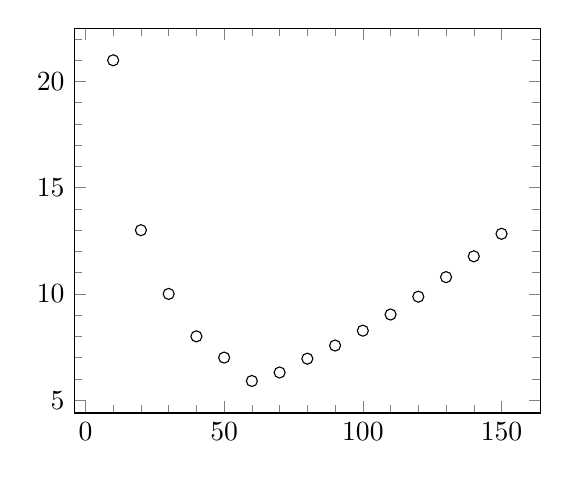
\begin{tikzpicture}
\begin{axis}[%
scatter/classes={%
    a={mark=o,draw=black}},
    minor y tick num = 4,
    minor x tick num = 4]
\addplot[scatter,only marks,%
    scatter src=explicit symbolic]%
table[meta=label] {
x y label
10 21.00 a
20 13.00 a
30 10.00 a
40 8.00 a
50 7.00 a
60 5.90 a
70 6.30 a
80 6.95 a
90 7.57 a
100 8.27 a
110 9.03 a
120 9.87 a
130 10.79 a
140 11.77 a
150 12.83 a
    };
\end{axis}
\end{tikzpicture}
\end{center}
\item[]
\item[]
In most cases, speed will affect the fuel consumption and therefore,
speed is the explanatory variable.

\item[]

\item[(b)]
It seems to be curved. More specifically, it looks like a parabolic
plot. It makes sense since if the speed is too low, the fuel
consumption goes up and same is for the very high speed.
For the optimal speed, however, which seems to be approximately
60, the fuel consumption seems to be very low (which is good).

\item[]

\item[(c)]
Unfortunately, there is no way describe variables as strictly
positively or negatively associated. The reason is that the
plot is parabolic and the association changes from negative
to positive. In other words, we have a mixed association.

\item[]

\item[(d)]
I would say it is reasonably strong since there are no points
that have a big deviation from the pattern. Also, the plot
represents quite tight rugby ball, which prompts us that the
relationship is strong.
\end{itemize}

\item[]
\item[]

\item[4.10]
\begin{itemize}
\item[(a)]
Below is the scatterplot for the data.

\item[]
\item[]
\begin{center}
\begin{tikzpicture}
\begin{axis}[%
scatter/classes={%
    a={mark=o,draw=black}},
    minor y tick num = 4,
    minor x tick num = 4]
\addplot[scatter,only marks,%
    scatter src=explicit symbolic]%
table[meta=label] {
x y label
29.68 0.42 a
29.87 2.58 a
30.16 2.68 a
30.22 2.60 a
30.48 2.48 a
30.65 2.38 a
30.90 2.26 a
    };
\end{axis}
\end{tikzpicture}
\end{center}
\item[]
\item[]
The temperature will have some effects on the coral growth.
Therefore, the temperature is an explanatory variable.

\item[]

\item[(b)]
The formula for $r$ is $r = \dfrac{1}{n - 1} \displaystyle\sum_{i = 1}^n \Big(\dfrac{x_i - \overline{x}}{s_x}\Big) \times \Big(\dfrac{y_i - \overline{y}}{s_y}\Big)$.\\\\
Therefore, we first need to find the averages for $x$ and $y$.
We get that $\overline{x} = 30.28$ and $\overline{y} \approx 2.51$.
We now need to find the standard deviations for $x$ and $y$.
We get $s_x \approx 0.42$ and $s_y \approx 0.15$.
Then we have:
\begin{align*}
&r = \dfrac{1}{n - 1} \displaystyle\sum_{i = 1}^n \Big(\dfrac{x_i - \overline{x}}{s_x}\Big) \times \Big(\dfrac{y_i - \overline{y}}{s_y}\Big)\\
&= \dfrac{1}{7 - 1} \displaystyle\sum_{i = 1}^n \Big(\dfrac{x_i - 30.28}{0.42}\Big) \times \Big(\dfrac{y_i - 2.51}{0.15}\Big)\\
&= \dfrac{1}{6} \times \Bigg(\Big(\dfrac{29.68 - 30.28}{0.42} \times \dfrac{2.63 - 2.51}{0.15}\Big) \times \Big(\dfrac{29.87 - 30.28}{0.42} \times \dfrac{2.58 - 2.51}{0.15}\Big)\\
&+ \Big(\dfrac{30.16 - 30.28}{0.42} \times \dfrac{2.68 - 2.51}{0.15}\Big) \times \Big(\dfrac{30.22 - 30.28}{0.42} \times \dfrac{2.60 - 2.51}{0.15}\Big)\\
&+ \Big(\dfrac{30.48 - 30.28}{0.42} \times \dfrac{2.48 - 2.51}{0.15}\Big) \times \Big(\dfrac{30.65 - 30.28}{0.42} \times \dfrac{2.38 - 2.51}{0.15}\Big)\\
&+ \Big(\dfrac{30.90 - 30.28}{0.42} \times \dfrac{2.26 - 2.51}{0.15}\Big)\Bigg)\\
&\approx\dfrac{1}{6} \big(-1.14 + (-0.45) + (-0.32) + (-0.08) + (-0.09) + (-0.76) + (-2.46)\big)\\
&\approx \dfrac{-5.3}{6} \approx -0.88.
\end{align*}
Finally, we got that $r = -0.13$. The correlation coefficient
shows that the plot gives us a negative linear pattern which
is easy to see in the plot of exercise (a).
\end{itemize}

\item[]
\item[]

\item[4.13]
Below is the scatterplot for the data.

\item[]
\item[]
\begin{center}
\begin{tikzpicture}
\begin{axis}[%
scatter/classes={%
    a={mark=o,draw=black}},
    minor y tick num = 4,
    minor x tick num = 4]
\addplot[scatter,only marks,%
    scatter src=explicit symbolic]%
table[meta=label] {
x y label
30 24 a
40 28 a
50 30 a
60 28 a
70 24 a
    };
\end{axis}
\end{tikzpicture}
\end{center}
\item[]
\item[]
Using the correlation calculator at \url{https://www.socscistatistics.com/tests/pearson/Default2.aspx},
we get that $r = 0$ (this is the verification, the problem does not
ask to do it by hand again). Although there is a strong relationship
between speed and mileage, the correlation is still 0 since the
shape of the scatterplot is not linear - it is curved. Correlation
can be used as a measure only in linear associations and since this
is not linear and rather curved, it does not make a lot of sense (other than maybe it is since the curve is half positive-half negative in terms
of slope of the line that approximates the branches ~ but generally speaking, still has nothing to do with it).

\item[]
\item[]

\item[4.37]
\begin{itemize}
\item[(a)]
Recall that the lower correlation, the lower association.
Therefore, Rachel should go with small-cap stocks because 0.21 < 0.50.

\item[]

\item[(b)]
She should look for a negative correlation (since the association between variables is negative).
\end{itemize}

\item[]
\item[]

\item[4.38]
The Psychologist talks about the correlation being 0 while
the newspaper reports that the correlation is negative.

\item[]
\item[]

\item[4.39]
\begin{itemize}
\item[(a)]
Sex is not a number.

\item[]

\item[(b)]
Correlation ranges from -1 to 1. Therefore, it cannot be 1.09 which
is larger than 1.

\item[]

\item[(c)]
Correlation is a unitless measure. Centimeter per kilogram is a unit
and therefore, the statement contains a blunder.
\end{itemize}

\end{itemize}

\end{document}
